\chapter{Application}\label{chpt:application}
\glsresetall

This chapter is about the application that was motivated in section~\ref{sec:intro:problem}. First of 
all the concept is specified. After that the acquisition of data as well as the implementation of the 
different components is described.

\section{Concept}\label{sec:app:concept}

The following concept is divided into two parts. The first part describes the productive application 
that transforms a Valorant video into another data representation using a pattern recognition 
algorithm. The second part covers all workflows to train a machine learning model that is used in the 
first part.

\subsection{Inference Application}\label{subsec:app:inference}

The productive application consists of five elements:

\begin{itemize}
	\item[\textbf{I1:}] Raw data
	\item[\textbf{I2:}] Data pre-processing
	\item[\textbf{I3:}] Neural network model
	\item[\textbf{I4:}] Post-processing algorithm
	\item[\textbf{I5:}] Transformed data representation
\end{itemize}

As raw data (I1) videos with Valorant gameplay are used. Those videos show a screen as depicted in 
figure~\ref{fig:intro:ingame}. Within this project the goal is to derive an alternative data 
representation (I5) that helps players and trainers to get a better overview of single rounds. 
Therefore it is important that the videos just contain individual rounds and not a whole match. This is 
secured in the data pre-processing step (I2). In order to generate a new representation that gives an 
overview, the data over time is summarized and presented as a single image (I5), like that in 
figure~\ref{fig:app:output}. However, only the information from the minimap in the upper left corner 
of the video is sufficient and due to training reasons, which are discussed in 
section~\ref{subsec:app:training}, this part of the map is also extracted during pre-processing (I2). 
The further steps are only performed on the cropped part of the video.

\begin{figure}
	\centering
	\includegraphics[width=0.8\linewidth]{images/05-output}
	\caption[Output representation as map.]{Output representation as map, summarizing all positions 
	of defender agents during one round on the map "Haven".}
	\label{fig:app:output}
\end{figure}

Image~\ref{fig:intro:minimap} shows different entities that could be possible targets of the detection 
algorithm~(I3). One possibility is just to find all players from one team without distinguishing the 
specific agent. The result of such an analysis is shown in figure~\ref{fig:app:output}. This is a graph 
that summarizes all positions of the defending team during a round on the already mentioned map 
"Haven". In a more advanced approach it is possible to detect the specific agents and create motion 
profiles for each of them. In addition, team or opponent abilities could also be recognized. It would 
be possible as well to combine those detection tasks and create various views to present the 
gathered data. The translation of the data from the video to the new representation is done by a 
neural network (I3). This is trained by the application described in section~\ref{subsec:app:training}. 
Finally a post-processing algorithm (I4) transforms the output data from the neural network into a 
better recognizable form of presentation (I5).

\subsection{Training Application}\label{subsec:app:training}

As written in section~\ref{subsec:app:inference} a trained neural network model is needed to 
transform a Valorant video into another form of representation. This part discusses a concept for an 
application that starts with raw data and outputs a trained machine learning model. That concept is 
outlined in figure~\ref{fig:app:conceptTrain} and differentiates between applications in purple, data 
in blue and programs in green.

For the acquiring of raw data multiple sources are available, in this concept called data platforms. 
From there the data has to be extracted for further usage. For this purpose an extractor is intended.
The most intuitive source is the game itself and everything that is rendered on the users screen. In 
that case the extractor is a screen capture device/program that records the screen and outputs a 
video. Other sources are already recorded videos, for example from gamers who upload their 
matches on Youtube for entertainment purposes. But Youtube is not the only platform: as in the 
introduction (Chapter~\ref{chpt:introduction}) mentioned especially during corona pandemic 
streaming platforms like Twitch~\cite{twitch} became a hype and there are many creators who live 
stream their Valorant gameplay. So this data could be captured directly while they are streaming or 
afterwards, because the streams are saved so that people can watch it again. In the case of available 
videos a download script is needed to get the data from the platforms.

\begin{figure}
	\centering
	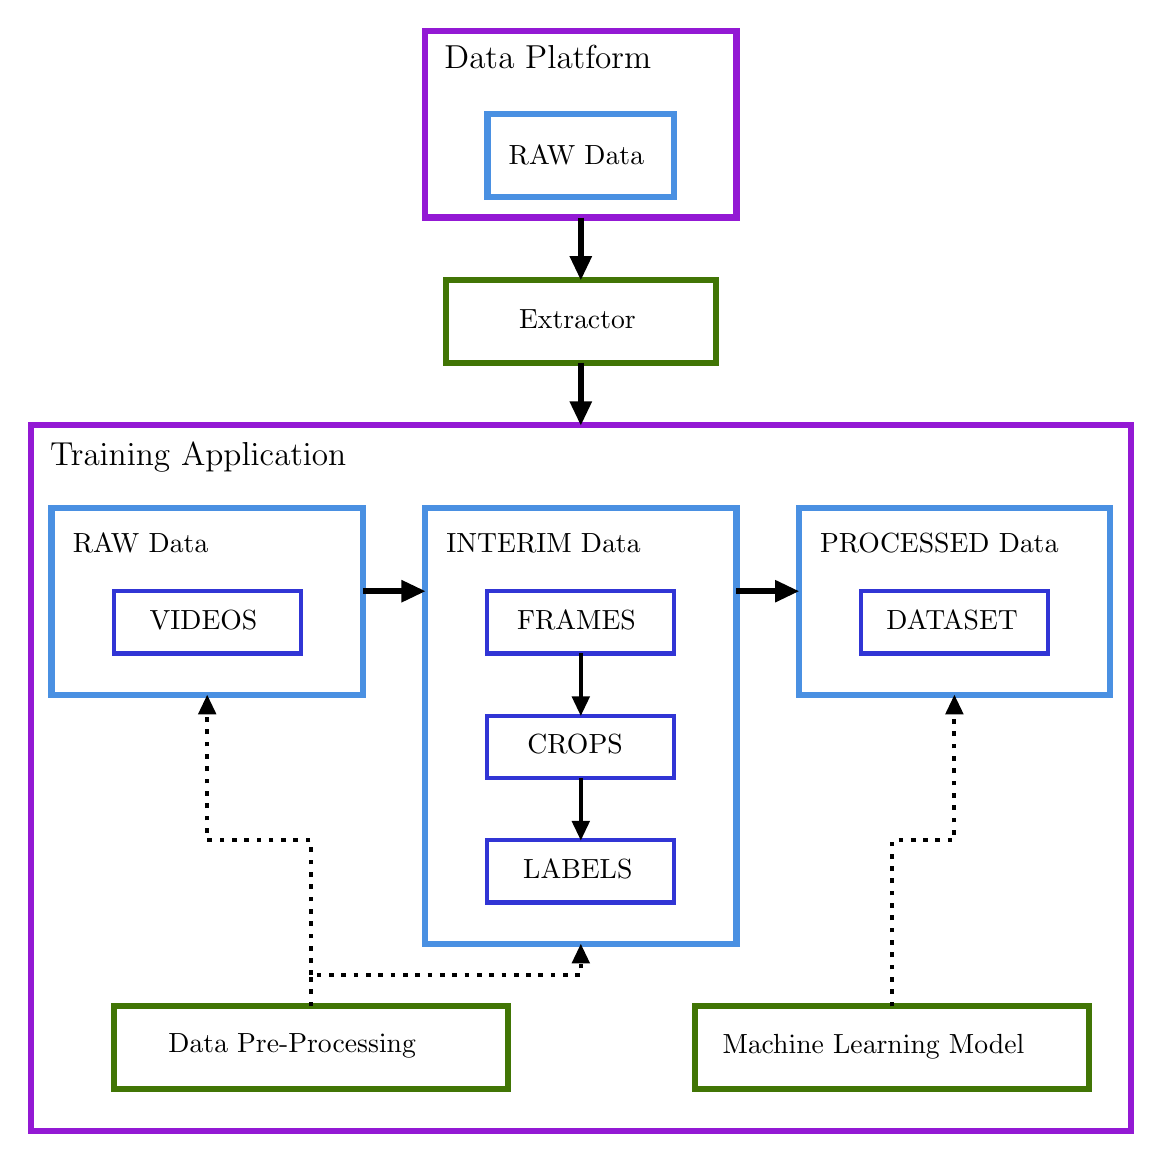
\begin{tikzpicture}[x=0.75pt,y=0.75pt,yscale=-1,xscale=1]
		\draw  [color={rgb, 255:red, 147; green, 25; blue, 212 }  ,draw opacity=1 ][line width=2.25]  
		(250,10) -- (400,10) -- (400,100) -- (250,100) -- cycle ;
		\draw  [color={rgb, 255:red, 147; green, 25; blue, 212 }  ,draw opacity=1 ][line width=2.25]  
		(60,200) -- (590,200) -- (590,540) -- (60,540) -- cycle ;
		\draw  [color={rgb, 255:red, 65; green, 117; blue, 5 }  ,draw opacity=1 ][line width=2.25]  
		(260,130) -- (390,130) -- (390,170) -- (260,170) -- cycle ;
		
		\draw [line width=2.25]    (325,100) -- (325,125) ;
		\draw [shift={(325,130)}, rotate = 270] [fill={rgb, 255:red, 0; green, 0; blue, 0 }  ][line 
		width=0.08]  [draw opacity=0] (11.43,-5.49) -- (0,0) -- (11.43,5.49) -- cycle    ;
		\draw [line width=2.25]    (325,170) -- (325,195) ;
		\draw [shift={(325,200)}, rotate = 270] [fill={rgb, 255:red, 0; green, 0; blue, 0 }  ][line 
		width=0.08]  [draw opacity=0] (11.43,-5.49) -- (0,0) -- (11.43,5.49) -- cycle    ;
		\draw  [color={rgb, 255:red, 74; green, 144; blue, 226 }  ,draw opacity=1 ][line width=2.25]  
		(70,240) -- (220,240) -- (220,330) -- (70,330) -- cycle ;
		\draw  [color={rgb, 255:red, 74; green, 144; blue, 226 }  ,draw opacity=1 ][line width=2.25]  
		(280,50) -- (370,50) -- (370,90) -- (280,90) -- cycle ;
		
		\draw  [color={rgb, 255:red, 65; green, 117; blue, 5 }  ,draw opacity=1 ][line width=2.25]  
		(100,480) -- (290,480) -- (290,520) -- (100,520) -- cycle ;
		
		\draw  [color={rgb, 255:red, 74; green, 144; blue, 226 }  ,draw opacity=1 ][line width=2.25]  
		(250,240) -- (400,240) -- (400,450) -- (250,450) -- cycle ;
		\draw  [color={rgb, 255:red, 49; green, 53; blue, 213 }  ,draw opacity=1 ][line width=1.5]  
		(100,280) -- (190,280) -- (190,310) -- (100,310) -- cycle ;
		\draw  [color={rgb, 255:red, 49; green, 53; blue, 213 }  ,draw opacity=1 ][line width=1.5]  
		(280,280) -- (370,280) -- (370,310) -- (280,310) -- cycle ;
		
		\draw  [color={rgb, 255:red, 49; green, 53; blue, 213 }  ,draw opacity=1 ][line width=1.5]  
		(280,340) -- (370,340) -- (370,370) -- (280,370) -- cycle ;
		
		\draw  [color={rgb, 255:red, 49; green, 53; blue, 213 }  ,draw opacity=1 ][line width=1.5]  
		(280,400) -- (370,400) -- (370,430) -- (280,430) -- cycle ;
		
		\draw [line width=1.5]    (325,310) -- (325,336) ;
		\draw [shift={(325,340)}, rotate = 270] [fill={rgb, 255:red, 0; green, 0; blue, 0 }  ][line 
		width=0.08]  [draw opacity=0] (9.29,-4.46) -- (0,0) -- (9.29,4.46) -- cycle    ;
		\draw [line width=1.5]    (325,370) -- (325,396) ;
		\draw [shift={(325,400)}, rotate = 270] [fill={rgb, 255:red, 0; green, 0; blue, 0 }  ][line 
		width=0.08]  [draw opacity=0] (9.29,-4.46) -- (0,0) -- (9.29,4.46) -- cycle    ;
		\draw [line width=2.25]    (220,280) -- (245,280) ;
		\draw [shift={(250,280)}, rotate = 180] [fill={rgb, 255:red, 0; green, 0; blue, 0 }  ][line 
		width=0.08]  [draw opacity=0] (11.43,-5.49) -- (0,0) -- (11.43,5.49) -- cycle    ;
		\draw  [color={rgb, 255:red, 74; green, 144; blue, 226 }  ,draw opacity=1 ][line width=2.25]  
		(430,240) -- (580,240) -- (580,330) -- (430,330) -- cycle ;
		\draw  [color={rgb, 255:red, 49; green, 53; blue, 213 }  ,draw opacity=1 ][line width=1.5]  
		(460,280) -- (550,280) -- (550,310) -- (460,310) -- cycle ;
		
		\draw [line width=2.25]    (400,280) -- (425,280) ;
		\draw [shift={(430,280)}, rotate = 180] [fill={rgb, 255:red, 0; green, 0; blue, 0 }  ][line 
		width=0.08]  [draw opacity=0] (11.43,-5.49) -- (0,0) -- (11.43,5.49) -- cycle    ;
		\draw  [color={rgb, 255:red, 65; green, 117; blue, 5 }  ,draw opacity=1 ][line width=2.25]  
		(380,480) -- (570,480) -- (570,520) -- (380,520) -- cycle ;
		
		\draw [line width=1.5]  [dash pattern={on 1.69pt off 2.76pt}]  (195,480) -- (195,465) -- 
		(325,465) -- (325,454) ;
		\draw [shift={(325,450)}, rotate = 90] [fill={rgb, 255:red, 0; green, 0; blue, 0 }  ][line 
		width=0.08]  [draw opacity=0] (9.29,-4.46) -- (0,0) -- (9.29,4.46) -- cycle    ;
		\draw [line width=1.5]  [dash pattern={on 1.69pt off 2.76pt}]  (195,465) -- (195,400) -- 
		(145,400) -- (145,334) ;
		\draw [shift={(145,330)}, rotate = 90] [fill={rgb, 255:red, 0; green, 0; blue, 0 }  ][line 
		width=0.08]  [draw opacity=0] (9.29,-4.46) -- (0,0) -- (9.29,4.46) -- cycle    ;
		\draw [line width=1.5]  [dash pattern={on 1.69pt off 2.76pt}]  (475,480) -- (475,400) -- 
		(505,400) -- (505,334) ;
		\draw [shift={(505,330)}, rotate = 90] [fill={rgb, 255:red, 0; green, 0; blue, 0 }  ][line 
		width=0.08]  [draw opacity=0] (9.29,-4.46) -- (0,0) -- (9.29,4.46) -- cycle    ;
		
		\draw (258,16) node [anchor=north west][inner sep=0.75pt]   [align=left] {{\large Data 
		Platform}};
		\draw (68,207) node [anchor=north west][inner sep=0.75pt]   [align=left] {{\large Training 
		Application}};
		\draw (289,64) node [anchor=north west][inner sep=0.75pt]   [align=left] {RAW Data};
		\draw (294,143) node [anchor=north west][inner sep=0.75pt]   [align=left] {Extractor};
		\draw (79,251) node [anchor=north west][inner sep=0.75pt]   [align=left] {RAW Data};
		\draw (259,251) node [anchor=north west][inner sep=0.75pt]   [align=left] {INTERIM Data};
		\draw (439,251) node [anchor=north west][inner sep=0.75pt]   [align=left] {PROCESSED Data};
		\draw (392,492) node [anchor=north west][inner sep=0.75pt]   [align=left] {Machine Learning 
		Model};
		\draw (116,288) node [anchor=north west][inner sep=0.75pt]   [align=left] {VIDEOS};
		\draw (471,288) node [anchor=north west][inner sep=0.75pt]   [align=left] {DATASET};
		\draw (293,288) node [anchor=north west][inner sep=0.75pt]   [align=left] {FRAMES};
		\draw (298,348) node [anchor=north west][inner sep=0.75pt]   [align=left] {CROPS};
		\draw (296,408) node [anchor=north west][inner sep=0.75pt]   [align=left] {LABELS};
		\draw (125,492) node [anchor=north west][inner sep=0.75pt]   [align=left] {Data 
		Pre-Processing};
	\end{tikzpicture}
	\caption{Concept for the training application.}
	\label{fig:app:conceptTrain}
\end{figure}

In the training application the acquired raw data is available in video format. In order to train a neural 
network several pre-processing steps are necessary to transform the raw data into a usable dataset. 
Therefore a data pre-processing component has to be built. The task of this module is to separate 
the video into individual frames, crop the frames onto the minimap, label the created images of the 
minimap and build a dataset. The pictures of the cropped minimap are reffered to as crops in the 
context of this project.

The first step of splitting the video into frames has to be made, because the neural network is 
trained with images even though inference is done on videos. The reason is that the annotation of 
images is easier than with videos. As noted in section~\ref{subsec:app:inference} the information 
from the minimap is sufficient and therefore the frames become cropped onto the minimap. That 
results in significant smaller images, which need less memory and a lot irrelevant and disturbing 
information is discarded. With the labeling step annotations are created that describe where 
detectable entities are in the image. These labels are used by the neural network as ground truth 
during training. Finally the crops and the labels are combined into a dataset that can be used by the 
machine learning model.

\section{Data}\label{sec:app:data}

This section describes the data that is actually used to carry out this project. Twitch serves as the 
data platform and a video~\cite{valVideo2023} of professionals playing at the Valorant 
Champions Tour 2023 in Los Angeles was downloaded. The chosen part of the video shows a match 
between the European team FNATIC and the American team LOUD. They played on three different 
maps (Ascent, Haven and Split). The video was downloaded with the tool yt-dlp~\cite{ytdlp2023} 
and the download script~\ref{lst:app:download}. 

\begin{minipage}{\linewidth}
	\vspace*{0.5cm}
	\begin{lstlisting}[language=Bash, keywordstyle=\color{black}, 
		caption=Download script to get the raw data., label=lst:app:download]
		#!/bin/bash
		
		s="$1"		# start timestamp
		e="$2"		# end timestamp
		n="$3"		# output name
		
		yt-dlp --external-downloader ffmpeg --external-downloader-args 
		"ffmpeg_i:-ss "$s".00 -to "$e".00" --output ""$n".mp4" 
		https://www.twitch.tv/videos/1907425469
	\end{lstlisting}
\end{minipage}

That script gets a start and an end timestamp and downloads the specified sequence of the selected 
video. With that technique the original video became downloaded without replays and 
non-gameplay. Consistent with the requirements the match was simultaneously split into single 
rounds. Therefore raw gameplay of three maps is available for further use within the project.

\begin{figure}
	\centering
	\includegraphics[width=0.7\linewidth]{images/06-input}
	\caption[Cropped input data.]{Cropped input data from the map "Haven".}
	\label{fig:app:input}
\end{figure}

The downloaded sequences show a different screen than depicted so far. The reason is that 
this video was part of the official sports reporting and therefore it is from observer view. The 
difference can be seen in figure~\ref{fig:app:input}. From players perspective only the agents of the 
same team and some enemy abilities can be seen on the minimap (see 
image~\ref{fig:intro:minimap}). The positions of opponents stay hidden. In contrast for spectators all 
players are visible on the map. That is advantageous for the learning task, because with that data the 
view of attackers and defenders can be trained at once. 

\section{YOLOv5}\label{sec:app:yolov5}

As machine learning model YOLOv5~\cite{jocher2020} was chosen because the usability of 
Ultralytics version is very good and feasibility already was proven. In addition, it is open source and 
continues to be actively developed~\cite{terven2023, river2021}. Furthermore with YOLOv5 
pre-trained checkpoints can be used for transfer learning~\cite{jocher2020}.

YOLOv5 is the first version that uses PyTorch~\cite{pytorch} instead of Darknet~\cite{darknet13} as 
machine learning framework. Both of them are open source and Darknet was developed by Joseph 
Redmon the first author of "You Only Look Once". While Darknet is written C and CUDA, PyTorch 
uses Python and makes training and testing easier for customized datasets~\cite{darknet13, 
pytorch, aydin2023, terven2023}. The architecture of YOLOv5 is divided into three parts: backbone, 
neck and head~\cite{archYolov5}. That is a common architecture of object 
detectors~\cite{terven2023}. 

In general the backbone is used to extract features from the input image and that is done with a 
\gls{acr-cnn}. Thereby earlier layers extract low-level features like edges and textures and deeper 
layers are used for detection of higher-level entities (object parts and semantic information). The 
neck connects the backbone and the head with additional convolutional layers, a \gls{acr-fpn} or 
other components that improve the feature representations from the backbone. Whilst the goal of 
the backbone is to capture features at different scales the focus of the neck is to enhance the spatial 
and semantic information across those different scales. The head makes the actual predictions on 
the provided features and mostly consists of several task-specific subnetworks for localization and 
classification. Predictions are made for each object candidate and in a post-processing step only the 
most confident detections are kept. A possible algorithm to filter out overlapping predictions is 
\gls{acr-nms}~\cite{terven2023}.

The backbone of YOLOv5 is a modified CSPDarknet53 a \gls{acr-cnn} with 53 convolutional 
layers~\cite{terven2023, redmon2018, wang2020}. It starts with a  layer that has a large window size 
(called stem) and has the goal to reduce memory and computational costs. Further each 
convolutional block consists of a convolutional layer followed by \gls{acr-bn} and a \gls{acr-silu} 
activation. The neck contains a \gls{acr-sppf} layer that processes the features at different scales 
and intends to speed up computation by pooling the different scaled features into a fixed-size 
feature map. Afterwards upsample layers increase the resolution of those feature 
maps~\cite{terven2023}. The complete architecture of YOLOv5 is depicted in 
figure~\ref{fig:aa:archyolov5}.

As mentioned before \gls{acr-nms} is a post-processing algorithm, with the goal to reduce the 
number of overlapping predictions. During detection the neural network generates so called 
bounding boxes to describe the location and size of an object~\cite{anchor2023}, but typically it is 
generating multiple boxes per entity and each bounding box has a different confidence score. 
\GLS{acr-nms} is used to filter out irrelevant bounding boxes by keeping just the most accurate per 
object. Therefore an \gls{acr-iou} and confidence threshold is defined for 
inference~\cite{terven2023}.

For training YOLOv5 can use data augmentation techniques, helping to improve the generalization 
ability and to reduce overfitting. The following two were used to train the experiments described in 
chapter~\ref{chpt:evaluation}. The first technique is called mosaic augmentation and thereby 
multiple images are combined into on large image with the goal to improve the handling of different 
object scales and translations. The second one is called HSV augmentation and randomly changes 
hue, saturation and value of the images and therefore creates a bigger variance in the learned 
data~\cite{archYolov5}.

Finally the training strategy AutoAnchor has to be described. This is an algorithm developed by 
Ultralytics~\cite{terven2023, archYolov5}. The training of YOLOv5 is based on anchor boxes with 
aim on improving the prediction quality. Later versions of YOLO did not need anchor boxes 
anymore~\cite{terven2023, zheng2022}. As mentioned before, the predictions of objects are based 
on bounding boxes, but unfortunately the objects have different shapes and sizes and so the boxes 
must have those too. For that so called anchors are used which are building a predefined set of 
bounding boxes with different shapes and sizes. The detection algorithm then has to decide which 
anchor matches best~\cite{anchor2023}. Ultralytics AutoAnchor algorithm is a pre-training tool that 
adjusts the predefined anchor boxes to better fit the ground truth boxes of custom 
datasets~\cite{terven2023, archYolov5}.

\section{Implementation}\label{sec:app:impl}

This section gives an overview of the realization of this project, starting from the point that the raw 
data is available as multiple videos showing single rounds of the game Valorant.

\section{Dataset}\label{sec:app:dataset}

\section{Summary}\label{sec:app:summary}
